\begin{figure}[t]
  \centering
  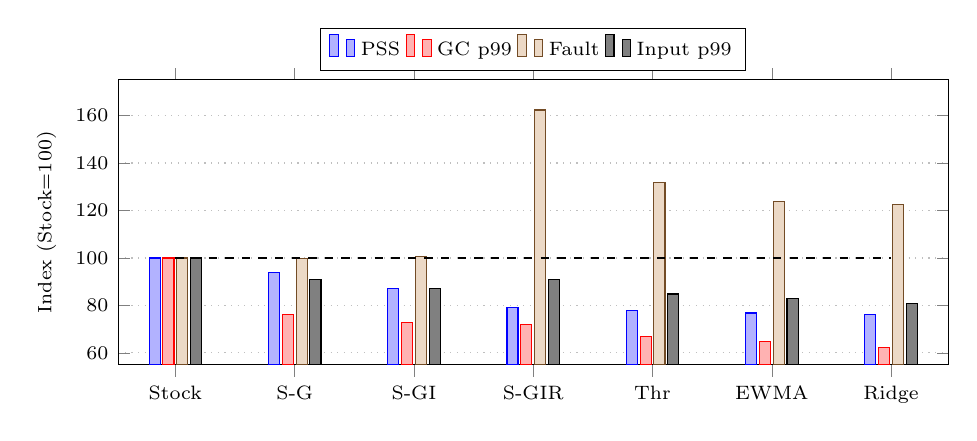
\begin{tikzpicture}
  \begin{axis}[
    width=\linewidth, height=5.2cm, ybar=1pt, bar width=4pt,
    ymin=55, ymax=175, symbolic x coords={Stock,S-G,S-GI,S-GIR,Thr,EWMA,Ridge}, xtick=data,
    x tick label style={font=\scriptsize}, ylabel={Index (Stock${=}100$)},
    ylabel style={font=\scriptsize}, ytick={60,80,100,120,140,160},
    tick label style={font=\scriptsize},
    legend style={font=\scriptsize, at={(0.5,1.03)}, anchor=south, legend columns=4},
    enlarge x limits=0.08, ymajorgrids, major grid style={dotted}]
  \addplot coordinates {(Stock,100.0) (S-G,94.0) (S-GI,87.0) (S-GIR,79.0) (Thr,77.9) (EWMA,76.8) (Ridge,76.1)};
  \addplot coordinates {(Stock,100.0) (S-G,76.2) (S-GI,72.7) (S-GIR,71.8) (Thr,67.0) (EWMA,64.7) (Ridge,62.4)};
  \addplot coordinates {(Stock,100.0) (S-G,99.9) (S-GI,100.6) (S-GIR,162.3) (Thr,131.7) (EWMA,123.8) (Ridge,122.7)};
  \addplot coordinates {(Stock,100.0) (S-G,90.8) (S-GI,87.3) (S-GIR,91.1) (Thr,84.8) (EWMA,82.8) (Ridge,81.0)};
  \draw[dashed] (axis cs:Stock,100) -- (axis cs:Ridge,100);
  \legend{PSS, GC p99, Fault, Input p99}
  \end{axis}
  \end{tikzpicture}
  \caption{Ablation ladder under the favorable workload (normalized policy
  indices, Stock${=}100$, mean of $n{=}30$ runs). Static heap and interop
  ($\textsf{S-G}\to\textsf{S-GI}$) lower PSS and GC tail with no fault cost;
  reclamation ($\textsf{S-GIR}$) reaches the lowest PSS but spikes the fault
  rate, which the online policies ($\textsf{Thr}/\textsf{EWMA}/\textsf{Ridge}$)
  pull back down while further improving input latency.}
  \label{fig:ablation}
\end{figure}

\begin{figure}[t]
  \centering
  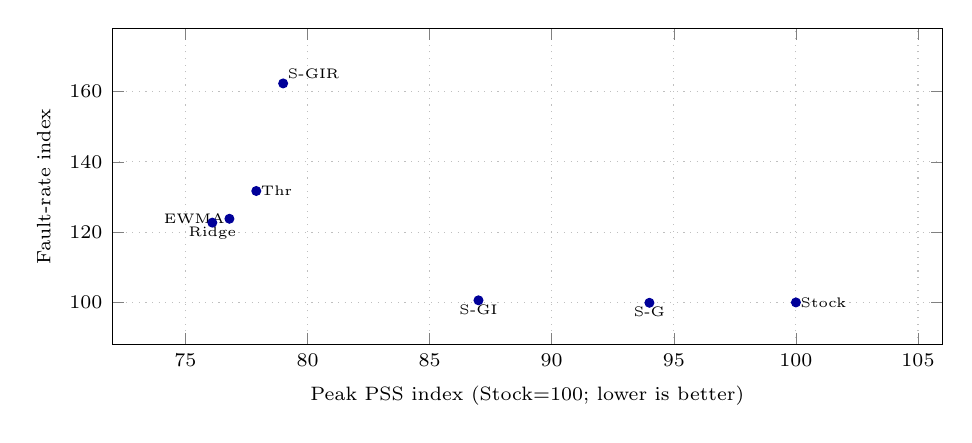
\begin{tikzpicture}
  \begin{axis}[
    width=\linewidth, height=5.6cm,
    xlabel={Peak PSS index (Stock${=}100$; lower is better)},
    ylabel={Fault-rate index}, xlabel style={font=\scriptsize},
    ylabel style={font=\scriptsize}, tick label style={font=\scriptsize},
    xmin=72, xmax=106, ymin=88, ymax=178, grid=both,
    major grid style={dotted}]
  \addplot[only marks, mark=*, mark size=1.6pt, color=blue!60!black]
    coordinates {(100.0,100.0) (94.0,99.9) (87.0,100.6) (79.0,162.3) (77.9,131.7) (76.8,123.8) (76.1,122.7)};
  \node[anchor=west, font=\tiny, inner sep=1.5pt] at (axis cs:100.0,100.0) {Stock};
  \node[anchor=north, font=\tiny, inner sep=1.5pt] at (axis cs:94.0,99.9) {S-G};
  \node[anchor=north, font=\tiny, inner sep=1.5pt] at (axis cs:87.0,100.6) {S-GI};
  \node[anchor=south west, font=\tiny, inner sep=1.5pt] at (axis cs:79.0,162.3) {S-GIR};
  \node[anchor=west, font=\tiny, inner sep=1.5pt] at (axis cs:77.9,131.7) {Thr};
  \node[anchor=east, font=\tiny, inner sep=1.5pt] at (axis cs:76.8,123.8) {EWMA};
  \node[anchor=north, font=\tiny, inner sep=1.5pt] at (axis cs:76.1,122.7) {Ridge};
  \end{axis}
  \end{tikzpicture}
  \caption{Footprint--refault tradeoff under the favorable workload. Static
  reclamation ($\textsf{S-GIR}$) buys the lowest PSS at a large refault
  penalty; the online controllers recover most of that penalty at nearly the
  same PSS, i.e.\ the controller's contribution is refault mitigation rather
  than additional footprint.}
  \label{fig:tradeoff}
\end{figure}

\begin{figure}[t]
  \centering
  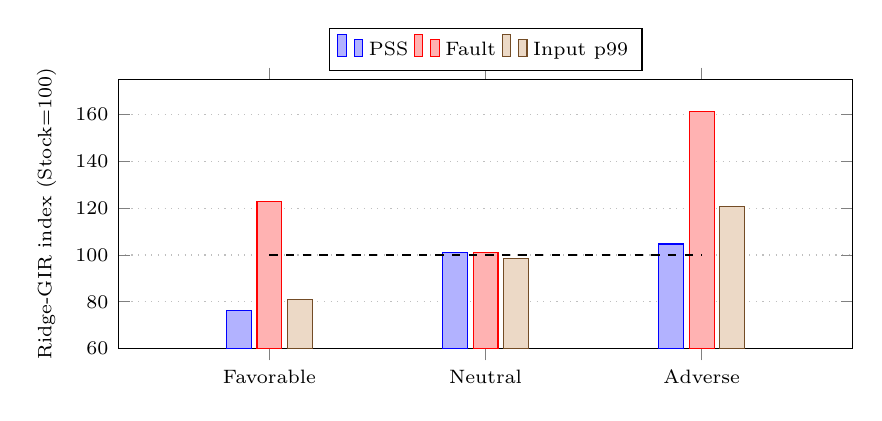
\begin{tikzpicture}
  \begin{axis}[
    width=0.9\linewidth, height=5.0cm, ybar=2pt, bar width=9pt,
    ymin=60, ymax=175, symbolic x coords={Favorable,Neutral,Adverse}, xtick=data,
    ylabel={Ridge-GIR index (Stock${=}100$)}, ylabel style={font=\scriptsize},
    tick label style={font=\scriptsize}, ytick={60,80,100,120,140,160},
    legend style={font=\scriptsize, at={(0.5,1.03)}, anchor=south, legend columns=3},
    enlarge x limits=0.35, ymajorgrids, major grid style={dotted}]
  \addplot coordinates {(Favorable,76.1) (Neutral,100.9) (Adverse,104.7)};
  \addplot coordinates {(Favorable,122.7) (Neutral,101.2) (Adverse,161.2)};
  \addplot coordinates {(Favorable,81.0) (Neutral,98.6) (Adverse,120.6)};
  \draw[dashed] (axis cs:Favorable,100) -- (axis cs:Adverse,100);
  \legend{PSS, Fault, Input p99}
  \end{axis}
  \end{tikzpicture}
  \caption{Cross-regime robustness of the coordinated learned policy
  ($\textsf{Ridge-GIR}$). Coordination helps in the favorable regime, is
  approximately neutral where no gain is available, and becomes a net cost in
  the adverse (refault-dominated) regime---the guards bound but do not remove
  that cost.}
  \label{fig:regimes}
\end{figure}
